%\documentclass[tikz, border=5pt]{standalone}
\usetikzlibrary{patterns} % 加载斜线阴影库
\begin{document}
	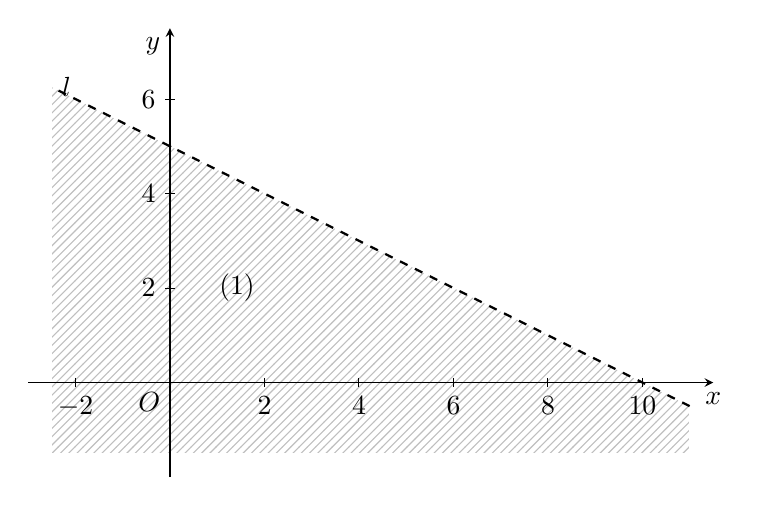
\begin{tikzpicture}[>=stealth, scale=0.6]
		
		% 4. 绘制阴影区域(东北斜线填充)位于最下层,
		\filldraw[pattern=north east lines, pattern color=gray!50] (-2.5, 6.25) -- (-2.5,-1.5) -- (11,-1.5) -- (11,-0.5)  ;
		\draw[white] (-2.5, 6.25) -- (-2.5,-1.5) -- (11,-1.5) -- (11,-0.5) ;
		
		% 1. 绘制坐标轴
		\draw[->] (-3,0) -- (11.5,0) node[below] {$x$}; % x轴(带箭头和标签)
		\draw[->] (0,-2) -- (0,7.5) node[below left] {$y$}; % y轴(带箭头和标签)
		\node at (0,0) [below left] {$O$};          % 原点标记
		
		% 绘制所有小刻度线(从 -1 到 2,每隔 1 单位画竖线)
		% 遍历x值,排除0刻度
		\foreach \x in {-2, 0,...,10} {
			\ifnum\x=0 % 若x=0,则不绘制刻度
			\else % 否则绘制刻度线和标签
			\draw (\x, 0.1) -- (\x, -0.1) node[below] {$\x$};
			\fi
		}
		
%		\foreach \x in {-2, 0,...,10} {
%			\draw (\x, 0.1) -- (\x, -0.1) node[below] {$\x$};  % 小竖线(长 0.2 单位)x轴刻度标记
%		}

		\foreach \y in {2,4,...,6} {
			\draw (0.1,\y) -- (-0.1,\y) node[left] {$\y$};  % 小竖线(长 0.2 单位)y轴刻度标记
		}
		
		% 2. 绘制直线  l 虚线 y=-x/2+5 
		\draw[dashed , thick] (11,-0.5) -- (-2.5, 6.25) node[ right] {$l$}; % 虚线部分
		
		% 3. 标记各点(A、B、C、B'、C')
		\fill (0,5) circle (1pt) ;
		
		\node at (2,2) [left] {$(1)$};
		
	\end{tikzpicture}
\end{document}
